\documentclass[twoside]{book}

% Packages required by doxygen
\usepackage{fixltx2e}
\usepackage{calc}
\usepackage{doxygen}
\usepackage[export]{adjustbox} % also loads graphicx
\usepackage{graphicx}
\usepackage[utf8]{inputenc}
\usepackage{makeidx}
\usepackage{multicol}
\usepackage{multirow}
\PassOptionsToPackage{warn}{textcomp}
\usepackage{textcomp}
\usepackage[nointegrals]{wasysym}
\usepackage[table]{xcolor}

% Font selection
\usepackage[T1]{fontenc}
\usepackage[scaled=.90]{helvet}
\usepackage{courier}
\usepackage{amssymb}
\usepackage{sectsty}
\renewcommand{\familydefault}{\sfdefault}
\allsectionsfont{%
  \fontseries{bc}\selectfont%
  \color{darkgray}%
}
\renewcommand{\DoxyLabelFont}{%
  \fontseries{bc}\selectfont%
  \color{darkgray}%
}
\newcommand{\+}{\discretionary{\mbox{\scriptsize$\hookleftarrow$}}{}{}}

% Page & text layout
\usepackage{geometry}
\geometry{%
  a4paper,%
  top=2.5cm,%
  bottom=2.5cm,%
  left=2.5cm,%
  right=2.5cm%
}
\tolerance=750
\hfuzz=15pt
\hbadness=750
\setlength{\emergencystretch}{15pt}
\setlength{\parindent}{0cm}
\setlength{\parskip}{0.2cm}
\makeatletter
\renewcommand{\paragraph}{%
  \@startsection{paragraph}{4}{0ex}{-1.0ex}{1.0ex}{%
    \normalfont\normalsize\bfseries\SS@parafont%
  }%
}
\renewcommand{\subparagraph}{%
  \@startsection{subparagraph}{5}{0ex}{-1.0ex}{1.0ex}{%
    \normalfont\normalsize\bfseries\SS@subparafont%
  }%
}
\makeatother

% Headers & footers
\usepackage{fancyhdr}
\pagestyle{fancyplain}
\fancyhead[LE]{\fancyplain{}{\bfseries\thepage}}
\fancyhead[CE]{\fancyplain{}{}}
\fancyhead[RE]{\fancyplain{}{\bfseries\leftmark}}
\fancyhead[LO]{\fancyplain{}{\bfseries\rightmark}}
\fancyhead[CO]{\fancyplain{}{}}
\fancyhead[RO]{\fancyplain{}{\bfseries\thepage}}
\fancyfoot[LE]{\fancyplain{}{}}
\fancyfoot[CE]{\fancyplain{}{}}
\fancyfoot[RE]{\fancyplain{}{\bfseries\scriptsize Generated on Tue Dec 29 2015 16\+:58\+:27 for Vgstools by Doxygen }}
\fancyfoot[LO]{\fancyplain{}{\bfseries\scriptsize Generated on Tue Dec 29 2015 16\+:58\+:27 for Vgstools by Doxygen }}
\fancyfoot[CO]{\fancyplain{}{}}
\fancyfoot[RO]{\fancyplain{}{}}
\renewcommand{\footrulewidth}{0.4pt}
\renewcommand{\chaptermark}[1]{%
  \markboth{#1}{}%
}
\renewcommand{\sectionmark}[1]{%
  \markright{\thesection\ #1}%
}

% Indices & bibliography
\usepackage{natbib}
\usepackage[titles]{tocloft}
\setcounter{tocdepth}{3}
\setcounter{secnumdepth}{5}
\makeindex

% Hyperlinks (required, but should be loaded last)
\usepackage{ifpdf}
\ifpdf
  \usepackage[pdftex,pagebackref=true]{hyperref}
\else
  \usepackage[ps2pdf,pagebackref=true]{hyperref}
\fi
\hypersetup{%
  colorlinks=true,%
  linkcolor=blue,%
  citecolor=blue,%
  unicode%
}

% Custom commands
\newcommand{\clearemptydoublepage}{%
  \newpage{\pagestyle{empty}\cleardoublepage}%
}


%===== C O N T E N T S =====

\begin{document}

% Titlepage & ToC
\hypersetup{pageanchor=false,
             bookmarks=true,
             bookmarksnumbered=true,
             pdfencoding=unicode
            }
\pagenumbering{roman}
\begin{titlepage}
\vspace*{7cm}
\begin{center}%
{\Large Vgstools }\\
\vspace*{1cm}
{\large Generated by Doxygen 1.8.9.1}\\
\vspace*{0.5cm}
{\small Tue Dec 29 2015 16:58:27}\\
\end{center}
\end{titlepage}
\clearemptydoublepage
\tableofcontents
\clearemptydoublepage
\pagenumbering{arabic}
\hypersetup{pageanchor=true}

%--- Begin generated contents ---
\chapter{Todo List}
\label{todo}
\hypertarget{todo}{}

\begin{DoxyRefList}
\item[\label{todo__todo000001}%
\hypertarget{todo__todo000001}{}%
Member \hyperlink{class_search_aab0de7f1b256ebfc720a5c9a26c7a5e4}{Search\+:\+:make\+Query} ()]\+: Make sure to retry untill not 500 on webbrequests as load errors happens.
\end{DoxyRefList}
\chapter{Hierarchical Index}
\section{Class Hierarchy}
This inheritance list is sorted roughly, but not completely, alphabetically\+:\begin{DoxyCompactList}
\item \contentsline{section}{Veganistan}{\pageref{class_veganistan}}{}
\begin{DoxyCompactList}
\item \contentsline{section}{News}{\pageref{class_news}}{}
\item \contentsline{section}{Search}{\pageref{class_search}}{}
\end{DoxyCompactList}
\end{DoxyCompactList}

\chapter{Class Index}
\section{Class List}
Here are the classes, structs, unions and interfaces with brief descriptions\+:\begin{DoxyCompactList}
\item\contentsline{section}{\hyperlink{class_news}{News} \\*This is the class that holds the news functions }{\pageref{class_news}}{}
\item\contentsline{section}{\hyperlink{class_search}{Search} \\*This is the class that holds the search functions }{\pageref{class_search}}{}
\item\contentsline{section}{\hyperlink{class_veganistan}{Veganistan} \\*This is the main class that holds the general functions and other classes inherits from }{\pageref{class_veganistan}}{}
\end{DoxyCompactList}

\chapter{File Index}
\section{File List}
Here is a list of all files with brief descriptions\+:\begin{DoxyCompactList}
\item\contentsline{section}{class/\hyperlink{news_8php}{news.\+php} \\*File containing the news class for vgstools }{\pageref{news_8php}}{}
\item\contentsline{section}{class/\hyperlink{search_8php}{search.\+php} \\*File containing the search class for vgstools }{\pageref{search_8php}}{}
\item\contentsline{section}{class/\hyperlink{veganistan_8php}{veganistan.\+php} \\*File containing the search class for vgstools }{\pageref{veganistan_8php}}{}
\end{DoxyCompactList}

\chapter{Class Documentation}
\hypertarget{class_news}{}\section{News Class Reference}
\label{class_news}\index{News@{News}}


This is the class that holds the news functions.  


Inheritance diagram for News\+:\begin{figure}[H]
\begin{center}
\leavevmode
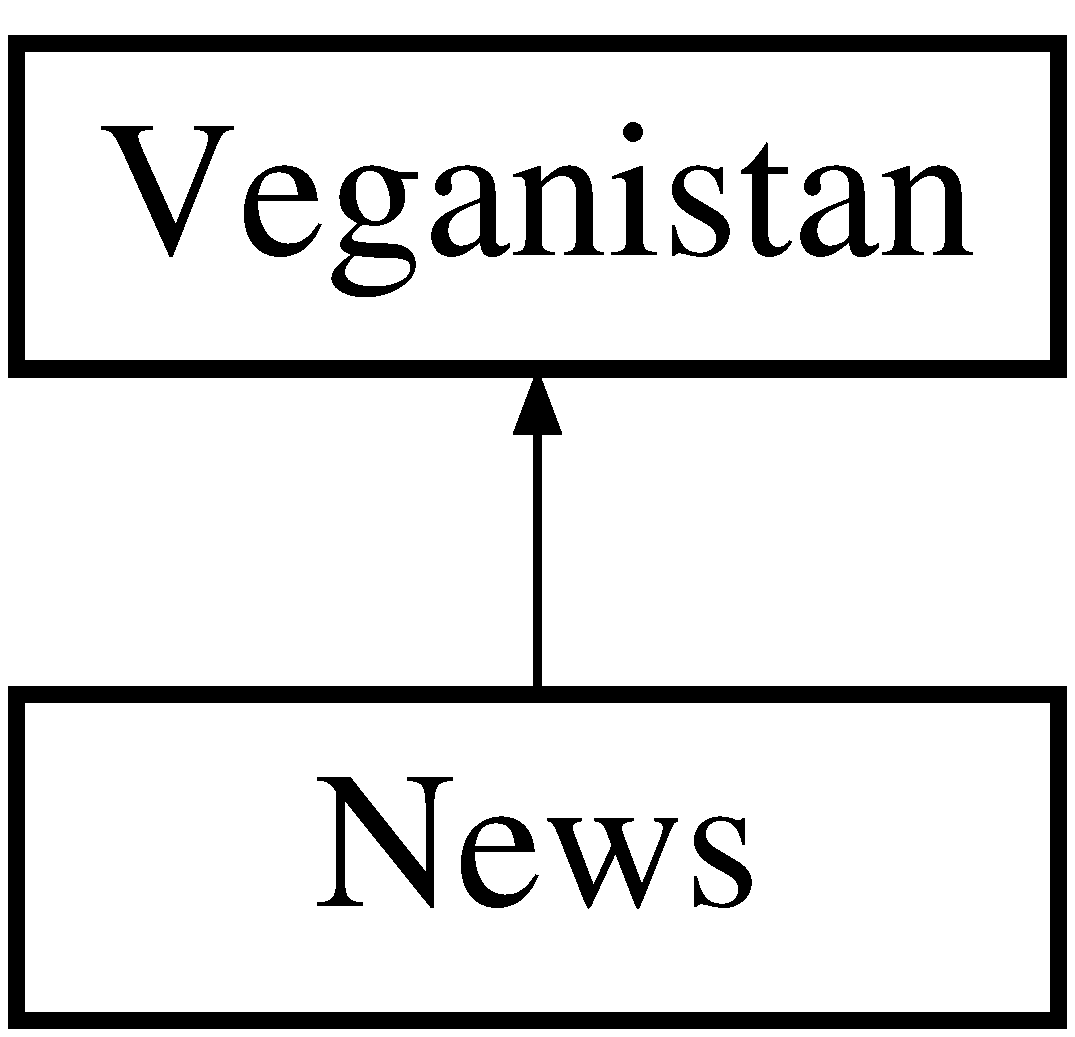
\includegraphics[height=2.000000cm]{class_news}
\end{center}
\end{figure}
\subsection*{Public Member Functions}
\begin{DoxyCompactItemize}
\item 
\hyperlink{class_news_ae09b063136b3d937ff18a3fbf59a1110}{get\+News\+X\+ML} (\$strict=F\+A\+L\+SE)
\begin{DoxyCompactList}\small\item\em Fetch the \hyperlink{class_news}{News} X\+ML feed. \end{DoxyCompactList}\end{DoxyCompactItemize}
\subsection*{Public Attributes}
\begin{DoxyCompactItemize}
\item 
\hyperlink{class_news_a7edd0e2bb0d22b388b300fbcfb1bf424}{\$town} = \char`\"{}\char`\"{}
\begin{DoxyCompactList}\small\item\em Town to find news for. \end{DoxyCompactList}\end{DoxyCompactItemize}
\subsection*{Private Member Functions}
\begin{DoxyCompactItemize}
\item 
\hyperlink{class_news_a1b0fb404a16f7b85f85b67eb05238b69}{is\+Town\+X\+ML} ()
\begin{DoxyCompactList}\small\item\em Check if X\+ML file name exists for specific town. \end{DoxyCompactList}\item 
\hyperlink{class_news_ad6eee22d2271aa0873387099a6a4c4c8}{xml\+\_\+exists} (\$path)
\begin{DoxyCompactList}\small\item\em Check so file is xml and exists. \end{DoxyCompactList}\item 
\hyperlink{class_news_aa9f1517421b0c0ecaeb992a00c3c37a8}{get\+X\+ML} (\$value=F\+A\+L\+SE)
\begin{DoxyCompactList}\small\item\em Get the X\+ML Value either for all or just a specific posttown. \end{DoxyCompactList}\item 
\hyperlink{class_news_a6b9d6856e5a51474160b2869ee690902}{sort\+Out\+Objects} (\$xmlfile, \$town\+\_\+array)
\begin{DoxyCompactList}\small\item\em Sort out objects that are in a posttown in the town area. \end{DoxyCompactList}\item 
\hyperlink{class_news_a002eef91ca7d8590faf45d61b84539c0}{is\+Link\+Town} (\$uri, \$towns)
\begin{DoxyCompactList}\small\item\em Function to look at link and match to post-\/town ,array used for non-\/strict search. \end{DoxyCompactList}\end{DoxyCompactItemize}


\subsection{Detailed Description}
This is the class that holds the news functions. 

\subsection{Member Function Documentation}
\hypertarget{class_news_ae09b063136b3d937ff18a3fbf59a1110}{}\label{class_news_ae09b063136b3d937ff18a3fbf59a1110} 
\index{News@{News}!get\+News\+X\+ML@{get\+News\+X\+ML}}
\index{get\+News\+X\+ML@{get\+News\+X\+ML}!News@{News}}
\subsubsection{\texorpdfstring{get\+News\+X\+M\+L()}{getNewsXML()}}
{\footnotesize\ttfamily News\+::get\+News\+X\+ML (\begin{DoxyParamCaption}\item[{}]{\$strict = {\ttfamily FALSE} }\end{DoxyParamCaption})}



Fetch the \hyperlink{class_news}{News} X\+ML feed. 


\begin{DoxyParams}[1]{Parameters}
bool & {\em \$strict,.} & Get strict from town if True otherwise look for posttown arrays for general area.\\
\hline
\end{DoxyParams}
\begin{DoxyReturn}{Returns}
Object. Returns simplexml objects for either all post towns in area or just the strict search ones. 
\end{DoxyReturn}
\hypertarget{class_news_aa9f1517421b0c0ecaeb992a00c3c37a8}{}\label{class_news_aa9f1517421b0c0ecaeb992a00c3c37a8} 
\index{News@{News}!get\+X\+ML@{get\+X\+ML}}
\index{get\+X\+ML@{get\+X\+ML}!News@{News}}
\subsubsection{\texorpdfstring{get\+X\+M\+L()}{getXML()}}
{\footnotesize\ttfamily News\+::get\+X\+ML (\begin{DoxyParamCaption}\item[{}]{\$value = {\ttfamily FALSE} }\end{DoxyParamCaption})\hspace{0.3cm}{\ttfamily [private]}}



Get the X\+ML Value either for all or just a specific posttown. 


\begin{DoxyParams}[1]{Parameters}
string & {\em \$value,.} & If set contains the town to check.\\
\hline
\end{DoxyParams}
\begin{DoxyReturn}{Returns}
mixed \$xml. Contains the Simple\+X\+ML object for a town or false if somethign went wrong and was not handled. 
\end{DoxyReturn}
\hypertarget{class_news_a002eef91ca7d8590faf45d61b84539c0}{}\label{class_news_a002eef91ca7d8590faf45d61b84539c0} 
\index{News@{News}!is\+Link\+Town@{is\+Link\+Town}}
\index{is\+Link\+Town@{is\+Link\+Town}!News@{News}}
\subsubsection{\texorpdfstring{is\+Link\+Town()}{isLinkTown()}}
{\footnotesize\ttfamily News\+::is\+Link\+Town (\begin{DoxyParamCaption}\item[{}]{\$uri,  }\item[{}]{\$towns }\end{DoxyParamCaption})\hspace{0.3cm}{\ttfamily [private]}}



Function to look at link and match to post-\/town ,array used for non-\/strict search. 


\begin{DoxyParams}[1]{Parameters}
string & {\em \$uri} & . The uri to get town from. \\
\hline
array & {\em \$towns,.} & The town array to compare with.\\
\hline
\end{DoxyParams}
\begin{DoxyReturn}{Returns}
bool. Return True if one of the post-\/towns is the town part of the link otherwise fasle. 
\end{DoxyReturn}
\hypertarget{class_news_a1b0fb404a16f7b85f85b67eb05238b69}{}\label{class_news_a1b0fb404a16f7b85f85b67eb05238b69} 
\index{News@{News}!is\+Town\+X\+ML@{is\+Town\+X\+ML}}
\index{is\+Town\+X\+ML@{is\+Town\+X\+ML}!News@{News}}
\subsubsection{\texorpdfstring{is\+Town\+X\+M\+L()}{isTownXML()}}
{\footnotesize\ttfamily News\+::is\+Town\+X\+ML (\begin{DoxyParamCaption}{ }\end{DoxyParamCaption})\hspace{0.3cm}{\ttfamily [private]}}



Check if X\+ML file name exists for specific town. 

\begin{DoxyReturn}{Returns}
bool. True if exists, False if not. 
\end{DoxyReturn}
\hypertarget{class_news_a6b9d6856e5a51474160b2869ee690902}{}\label{class_news_a6b9d6856e5a51474160b2869ee690902} 
\index{News@{News}!sort\+Out\+Objects@{sort\+Out\+Objects}}
\index{sort\+Out\+Objects@{sort\+Out\+Objects}!News@{News}}
\subsubsection{\texorpdfstring{sort\+Out\+Objects()}{sortOutObjects()}}
{\footnotesize\ttfamily News\+::sort\+Out\+Objects (\begin{DoxyParamCaption}\item[{}]{\$xmlfile,  }\item[{}]{\$town\+\_\+array }\end{DoxyParamCaption})\hspace{0.3cm}{\ttfamily [private]}}



Sort out objects that are in a posttown in the town area. 


\begin{DoxyParams}[1]{Parameters}
Objct & {\em \$xmlfile,.} & The raw simplexml feed from xml file. \\
\hline
array & {\em \$town\+\_\+array,.} & The acctuall array of towns to compare with.\\
\hline
\end{DoxyParams}
\begin{DoxyReturn}{Returns}
array \$output. Array containing objects of place data in pure text. 
\end{DoxyReturn}
\hypertarget{class_news_ad6eee22d2271aa0873387099a6a4c4c8}{}\label{class_news_ad6eee22d2271aa0873387099a6a4c4c8} 
\index{News@{News}!xml\+\_\+exists@{xml\+\_\+exists}}
\index{xml\+\_\+exists@{xml\+\_\+exists}!News@{News}}
\subsubsection{\texorpdfstring{xml\+\_\+exists()}{xml\_exists()}}
{\footnotesize\ttfamily News\+::xml\+\_\+exists (\begin{DoxyParamCaption}\item[{}]{\$path }\end{DoxyParamCaption})\hspace{0.3cm}{\ttfamily [private]}}



Check so file is xml and exists. 


\begin{DoxyParams}[1]{Parameters}
string & {\em \$path,.} & The path to check.\\
\hline
\end{DoxyParams}
\$return bool. True if file exists and is X\+ML otherwise F\+A\+L\+SE. 

\subsection{Member Data Documentation}
\hypertarget{class_news_a7edd0e2bb0d22b388b300fbcfb1bf424}{}\label{class_news_a7edd0e2bb0d22b388b300fbcfb1bf424} 
\index{News@{News}!\$town@{\$town}}
\index{\$town@{\$town}!News@{News}}
\subsubsection{\texorpdfstring{\$town}{$town}}
{\footnotesize\ttfamily News\+::\$town = \char`\"{}\char`\"{}}



Town to find news for. 



The documentation for this class was generated from the following file\+:\begin{DoxyCompactItemize}
\item 
class/\hyperlink{news_8php}{news.\+php}\end{DoxyCompactItemize}

\hypertarget{class_search}{}\section{Search Class Reference}
\label{class_search}\index{Search@{Search}}


This is the class that holds the search functions.  


Inheritance diagram for Search\+:\begin{figure}[H]
\begin{center}
\leavevmode
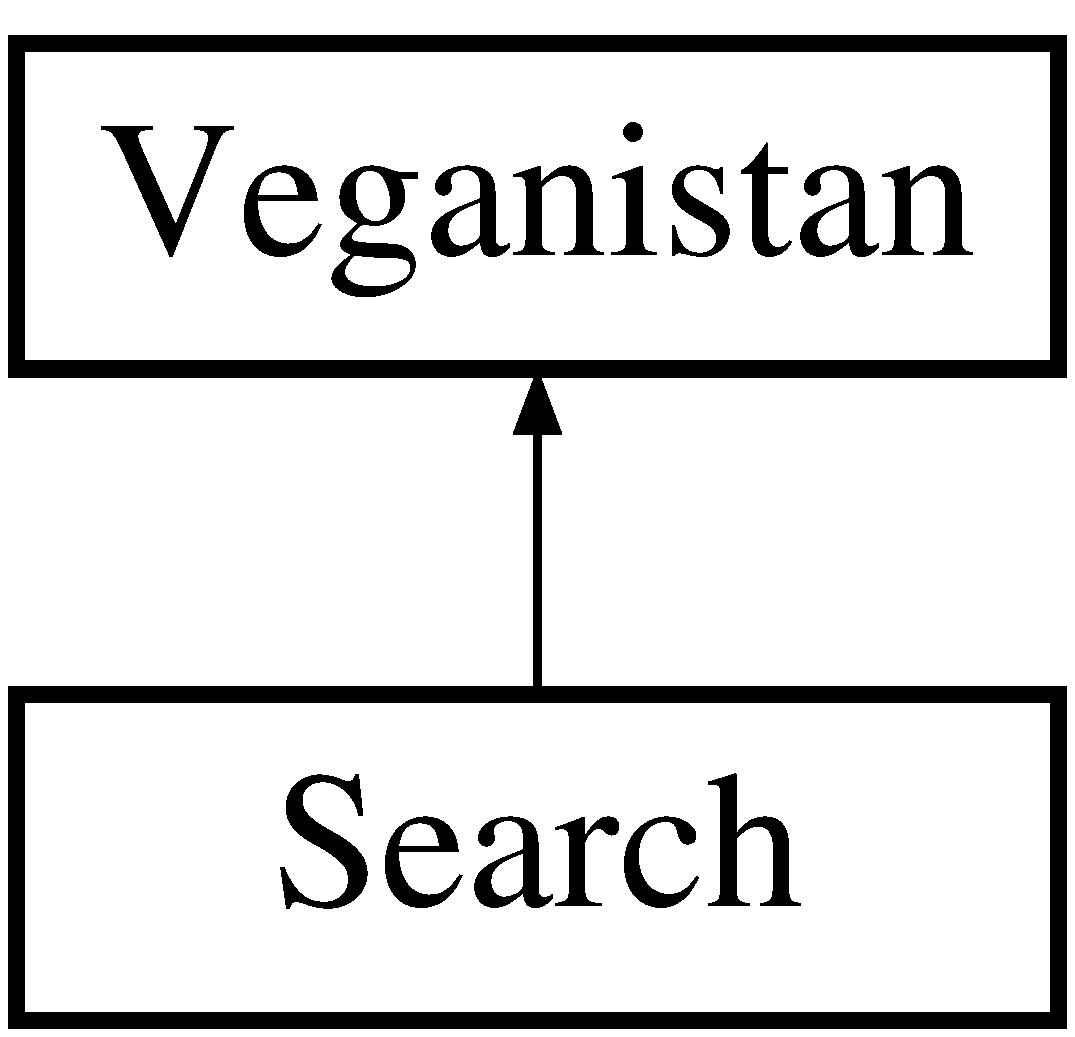
\includegraphics[height=2.000000cm]{class_search}
\end{center}
\end{figure}
\subsection*{Public Member Functions}
\begin{DoxyCompactItemize}
\item 
\hyperlink{class_search_a80725b6a32dfc685558764d47002d9c0}{\+\_\+search} ()
\begin{DoxyCompactList}\small\item\em Do the acctual search based on if the strict property is T\+R\+U\+E O\+R F\+A\+L\+S\+E. \end{DoxyCompactList}\end{DoxyCompactItemize}
\subsection*{Public Attributes}
\begin{DoxyCompactItemize}
\item 
\hyperlink{class_search_ad5a555c9913e06e21914adb4d9fc36d6}{\$strict} = F\+A\+L\+S\+E
\begin{DoxyCompactList}\small\item\em Defines if search should be strict or not. \end{DoxyCompactList}\item 
\hyperlink{class_search_aab54895afb81d800b1aa7b5ed1e316d2}{\$town} = \char`\"{}\char`\"{}
\begin{DoxyCompactList}\small\item\em The town to work with. \end{DoxyCompactList}\end{DoxyCompactItemize}
\subsection*{Protected Attributes}
\begin{DoxyCompactItemize}
\item 
\hyperlink{class_search_adbc71d7a9ff28a661af822ca70dfeefa}{\$search\+\_\+uri} = \char`\"{}http\+://www.\+veganistan.\+se/?field\+\_\+adress\+\_\+locality=\char`\"{}
\begin{DoxyCompactList}\small\item\em \hyperlink{class_search}{Search} U\+R\+I. \end{DoxyCompactList}\item 
\hyperlink{class_search_a0bdf2816de59f8db308bc03285152358}{\$search\+Town} = \char`\"{}\char`\"{}
\begin{DoxyCompactList}\small\item\em The current town being searched when generous search is used. \end{DoxyCompactList}\end{DoxyCompactItemize}
\subsection*{Private Member Functions}
\begin{DoxyCompactItemize}
\item 
\hyperlink{class_search_a6469a0900a719795f117999646e78670}{exact\+Search} ()
\begin{DoxyCompactList}\small\item\em Run an search for jsut the current town. \end{DoxyCompactList}\item 
\hyperlink{class_search_ac7ab4b286f468dbc67184e3d8e2ec086}{generous\+Search} ()
\begin{DoxyCompactList}\small\item\em Make an generous search by going through all towns in town array and querying them. \end{DoxyCompactList}\item 
\hyperlink{class_search_aab0de7f1b256ebfc720a5c9a26c7a5e4}{make\+Query} ()
\begin{DoxyCompactList}\small\item\em Make the acctual query to the homepage. \end{DoxyCompactList}\item 
\hyperlink{class_search_ac74e4ae4005b43140ce27fa3be53803a}{get\+Links} ()
\begin{DoxyCompactList}\small\item\em Get all links for a search. \end{DoxyCompactList}\item 
\hyperlink{class_search_a0b07d40d538cc7c3f49e2906da900759}{get\+Links\+From\+Page} (\$content)
\begin{DoxyCompactList}\small\item\em Fetch the acctual links to resturants from a string (mostly the content result of a search). \end{DoxyCompactList}\item 
\hyperlink{class_search_a0ae3fdf6e8c01b665dbbfd3cb5afd82e}{fetch\+Links\+From\+Page} (\$uri)
\begin{DoxyCompactList}\small\item\em Fetch the content of a page and then send it to get\+Links\+From\+Page method to extrapolate links. \end{DoxyCompactList}\item 
\hyperlink{class_search_ada895dffcd96b9471758c63f17363df1}{is\+Multi\+Page} (\$content)
\begin{DoxyCompactList}\small\item\em Look at a string and see if it is multipage html-\/page by looking for pager class. \end{DoxyCompactList}\item 
\hyperlink{class_search_acb6f51d3e3311922bec40d096b0bac99}{amount\+Pages} (\$content)
\begin{DoxyCompactList}\small\item\em Fetch the content and count if it is multipage by looking for the last number in the description of page length. \end{DoxyCompactList}\end{DoxyCompactItemize}


\subsection{Detailed Description}
This is the class that holds the search functions. 

\subsection{Member Function Documentation}
\hypertarget{class_search_a80725b6a32dfc685558764d47002d9c0}{}\index{Search@{Search}!\+\_\+search@{\+\_\+search}}
\index{\+\_\+search@{\+\_\+search}!Search@{Search}}
\subsubsection[{\+\_\+search}]{\setlength{\rightskip}{0pt plus 5cm}Search\+::\+\_\+search (
\begin{DoxyParamCaption}
{}
\end{DoxyParamCaption}
)}\label{class_search_a80725b6a32dfc685558764d47002d9c0}


Do the acctual search based on if the strict property is T\+R\+U\+E O\+R F\+A\+L\+S\+E. 

\begin{DoxyReturn}{Returns}
Array Returns an array with the result. 
\end{DoxyReturn}
\hypertarget{class_search_acb6f51d3e3311922bec40d096b0bac99}{}\index{Search@{Search}!amount\+Pages@{amount\+Pages}}
\index{amount\+Pages@{amount\+Pages}!Search@{Search}}
\subsubsection[{amount\+Pages}]{\setlength{\rightskip}{0pt plus 5cm}Search\+::amount\+Pages (
\begin{DoxyParamCaption}
\item[{}]{\$content}
\end{DoxyParamCaption}
)\hspace{0.3cm}{\ttfamily [private]}}\label{class_search_acb6f51d3e3311922bec40d096b0bac99}


Fetch the content and count if it is multipage by looking for the last number in the description of page length. 


\begin{DoxyParams}{Parameters}
{\em \$content} & String Contains the H\+T\+M\+L code of an U\+R\+I to check how many pages it is.\\
\hline
\end{DoxyParams}
\begin{DoxyReturn}{Returns}
Integer Number of pages in pagination. 
\end{DoxyReturn}
\hypertarget{class_search_a6469a0900a719795f117999646e78670}{}\index{Search@{Search}!exact\+Search@{exact\+Search}}
\index{exact\+Search@{exact\+Search}!Search@{Search}}
\subsubsection[{exact\+Search}]{\setlength{\rightskip}{0pt plus 5cm}Search\+::exact\+Search (
\begin{DoxyParamCaption}
{}
\end{DoxyParamCaption}
)\hspace{0.3cm}{\ttfamily [private]}}\label{class_search_a6469a0900a719795f117999646e78670}


Run an search for jsut the current town. 

\begin{DoxyReturn}{Returns}
Array containing the result of search. 
\end{DoxyReturn}
\hypertarget{class_search_a0ae3fdf6e8c01b665dbbfd3cb5afd82e}{}\index{Search@{Search}!fetch\+Links\+From\+Page@{fetch\+Links\+From\+Page}}
\index{fetch\+Links\+From\+Page@{fetch\+Links\+From\+Page}!Search@{Search}}
\subsubsection[{fetch\+Links\+From\+Page}]{\setlength{\rightskip}{0pt plus 5cm}Search\+::fetch\+Links\+From\+Page (
\begin{DoxyParamCaption}
\item[{}]{\$uri}
\end{DoxyParamCaption}
)\hspace{0.3cm}{\ttfamily [private]}}\label{class_search_a0ae3fdf6e8c01b665dbbfd3cb5afd82e}


Fetch the content of a page and then send it to get\+Links\+From\+Page method to extrapolate links. 


\begin{DoxyParams}{Parameters}
{\em \$uri} & String The U\+R\+I string to load the content off. \\
\hline
\end{DoxyParams}
\begin{DoxyReturn}{Returns}
Array containing the links found on the \$uri page or F\+A\+L\+S\+E if none is found or anything goes wrong. 
\end{DoxyReturn}
\hypertarget{class_search_ac7ab4b286f468dbc67184e3d8e2ec086}{}\index{Search@{Search}!generous\+Search@{generous\+Search}}
\index{generous\+Search@{generous\+Search}!Search@{Search}}
\subsubsection[{generous\+Search}]{\setlength{\rightskip}{0pt plus 5cm}Search\+::generous\+Search (
\begin{DoxyParamCaption}
{}
\end{DoxyParamCaption}
)\hspace{0.3cm}{\ttfamily [private]}}\label{class_search_ac7ab4b286f468dbc67184e3d8e2ec086}


Make an generous search by going through all towns in town array and querying them. 

\begin{DoxyReturn}{Returns}
Array with data found in search or F\+A\+L\+S\+E if nothing is found. 
\end{DoxyReturn}
\hypertarget{class_search_ac74e4ae4005b43140ce27fa3be53803a}{}\index{Search@{Search}!get\+Links@{get\+Links}}
\index{get\+Links@{get\+Links}!Search@{Search}}
\subsubsection[{get\+Links}]{\setlength{\rightskip}{0pt plus 5cm}Search\+::get\+Links (
\begin{DoxyParamCaption}
{}
\end{DoxyParamCaption}
)\hspace{0.3cm}{\ttfamily [private]}}\label{class_search_ac74e4ae4005b43140ce27fa3be53803a}


Get all links for a search. 

\begin{DoxyReturn}{Returns}
Returns an spl\+Fixed\+Array of all resturant urls on multiple pages if the search resulted in an multipage answer or an array of urls if not multipage and F\+A\+L\+S\+E on error. 
\end{DoxyReturn}
\hypertarget{class_search_a0b07d40d538cc7c3f49e2906da900759}{}\index{Search@{Search}!get\+Links\+From\+Page@{get\+Links\+From\+Page}}
\index{get\+Links\+From\+Page@{get\+Links\+From\+Page}!Search@{Search}}
\subsubsection[{get\+Links\+From\+Page}]{\setlength{\rightskip}{0pt plus 5cm}Search\+::get\+Links\+From\+Page (
\begin{DoxyParamCaption}
\item[{}]{\$content}
\end{DoxyParamCaption}
)\hspace{0.3cm}{\ttfamily [private]}}\label{class_search_a0b07d40d538cc7c3f49e2906da900759}


Fetch the acctual links to resturants from a string (mostly the content result of a search). 


\begin{DoxyParams}{Parameters}
{\em \$content} & String that contains the H\+T\+M\+L result of a search. \\
\hline
\end{DoxyParams}
\begin{DoxyReturn}{Returns}
Either an array of links to resturants or F\+A\+L\+S\+E if none is found or something goes wrong. 
\end{DoxyReturn}
\hypertarget{class_search_ada895dffcd96b9471758c63f17363df1}{}\index{Search@{Search}!is\+Multi\+Page@{is\+Multi\+Page}}
\index{is\+Multi\+Page@{is\+Multi\+Page}!Search@{Search}}
\subsubsection[{is\+Multi\+Page}]{\setlength{\rightskip}{0pt plus 5cm}Search\+::is\+Multi\+Page (
\begin{DoxyParamCaption}
\item[{}]{\$content}
\end{DoxyParamCaption}
)\hspace{0.3cm}{\ttfamily [private]}}\label{class_search_ada895dffcd96b9471758c63f17363df1}


Look at a string and see if it is multipage html-\/page by looking for pager class. 


\begin{DoxyParams}{Parameters}
{\em \$content} & String Contains the H\+T\+M\+L code of an U\+R\+I to check if it is a multipage reuslt.\\
\hline
\end{DoxyParams}
\begin{DoxyReturn}{Returns}
Bool True if it is multipage otherwise F\+A\+L\+S\+E. 
\end{DoxyReturn}
\hypertarget{class_search_aab0de7f1b256ebfc720a5c9a26c7a5e4}{}\index{Search@{Search}!make\+Query@{make\+Query}}
\index{make\+Query@{make\+Query}!Search@{Search}}
\subsubsection[{make\+Query}]{\setlength{\rightskip}{0pt plus 5cm}Search\+::make\+Query (
\begin{DoxyParamCaption}
{}
\end{DoxyParamCaption}
)\hspace{0.3cm}{\ttfamily [private]}}\label{class_search_aab0de7f1b256ebfc720a5c9a26c7a5e4}


Make the acctual query to the homepage. 

\begin{DoxyRefDesc}{Todo}
\item[\hyperlink{todo__todo000001}{Todo}]\+: Make sure to retry untill not 500 on webbrequests as load errors happens.\end{DoxyRefDesc}


\begin{DoxyReturn}{Returns}
spl\+Fixed\+Array for each place found containg an Spl\+Fixed\+Array of three rows with Name, address and description as there content or bool F\+A\+L\+S\+E if something fails. 
\end{DoxyReturn}


\subsection{Member Data Documentation}
\hypertarget{class_search_adbc71d7a9ff28a661af822ca70dfeefa}{}\index{Search@{Search}!\$search\+\_\+uri@{\$search\+\_\+uri}}
\index{\$search\+\_\+uri@{\$search\+\_\+uri}!Search@{Search}}
\subsubsection[{\$search\+\_\+uri}]{\setlength{\rightskip}{0pt plus 5cm}Search\+::\$search\+\_\+uri = \char`\"{}http\+://www.\+veganistan.\+se/?field\+\_\+adress\+\_\+locality=\char`\"{}\hspace{0.3cm}{\ttfamily [protected]}}\label{class_search_adbc71d7a9ff28a661af822ca70dfeefa}


\hyperlink{class_search}{Search} U\+R\+I. 

\hypertarget{class_search_a0bdf2816de59f8db308bc03285152358}{}\index{Search@{Search}!\$search\+Town@{\$search\+Town}}
\index{\$search\+Town@{\$search\+Town}!Search@{Search}}
\subsubsection[{\$search\+Town}]{\setlength{\rightskip}{0pt plus 5cm}Search\+::\$search\+Town = \char`\"{}\char`\"{}\hspace{0.3cm}{\ttfamily [protected]}}\label{class_search_a0bdf2816de59f8db308bc03285152358}


The current town being searched when generous search is used. 

\hypertarget{class_search_ad5a555c9913e06e21914adb4d9fc36d6}{}\index{Search@{Search}!\$strict@{\$strict}}
\index{\$strict@{\$strict}!Search@{Search}}
\subsubsection[{\$strict}]{\setlength{\rightskip}{0pt plus 5cm}Search\+::\$strict = F\+A\+L\+S\+E}\label{class_search_ad5a555c9913e06e21914adb4d9fc36d6}


Defines if search should be strict or not. 

\hypertarget{class_search_aab54895afb81d800b1aa7b5ed1e316d2}{}\index{Search@{Search}!\$town@{\$town}}
\index{\$town@{\$town}!Search@{Search}}
\subsubsection[{\$town}]{\setlength{\rightskip}{0pt plus 5cm}Search\+::\$town = \char`\"{}\char`\"{}}\label{class_search_aab54895afb81d800b1aa7b5ed1e316d2}


The town to work with. 



The documentation for this class was generated from the following file\+:\begin{DoxyCompactItemize}
\item 
class/\hyperlink{search_8php}{search.\+php}\end{DoxyCompactItemize}

\hypertarget{class_veganistan}{}\section{Veganistan Class Reference}
\label{class_veganistan}\index{Veganistan@{Veganistan}}


This is the main class that holds the general functions and other classes inherits from.  


Inheritance diagram for Veganistan\+:\begin{figure}[H]
\begin{center}
\leavevmode
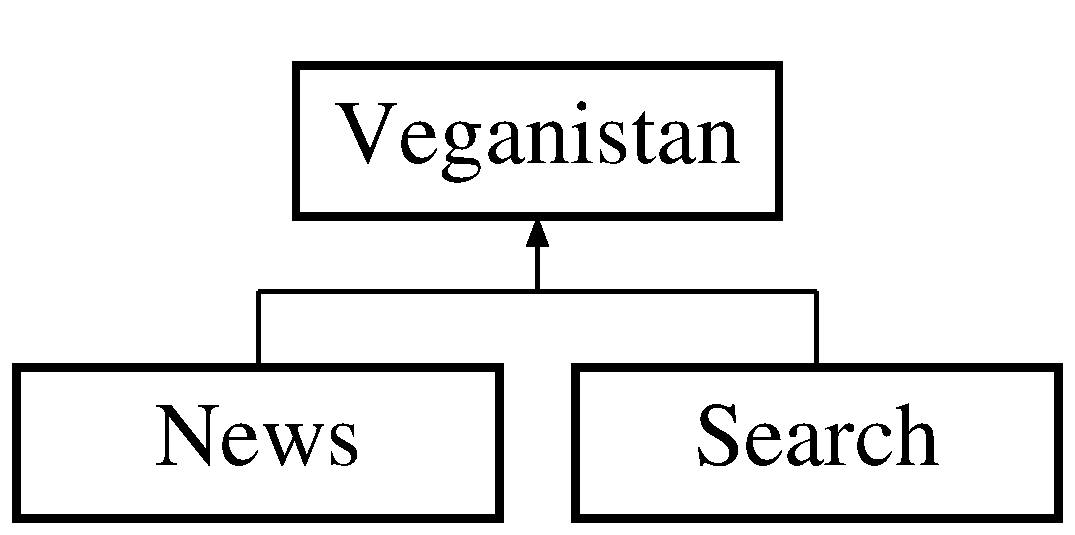
\includegraphics[height=2.000000cm]{class_veganistan}
\end{center}
\end{figure}


\subsection{Detailed Description}
This is the main class that holds the general functions and other classes inherits from. 

The documentation for this class was generated from the following file\+:\begin{DoxyCompactItemize}
\item 
class/\hyperlink{veganistan_8php}{veganistan.\+php}\end{DoxyCompactItemize}

\chapter{File Documentation}
\hypertarget{news_8php}{}\section{class/news.php File Reference}
\label{news_8php}\index{class/news.\+php@{class/news.\+php}}


File containing the news class for vgstools.  


\subsection*{Classes}
\begin{DoxyCompactItemize}
\item 
class \hyperlink{class_news}{News}
\begin{DoxyCompactList}\small\item\em This is the class that holds the news functions. \end{DoxyCompactList}\end{DoxyCompactItemize}


\subsection{Detailed Description}
File containing the news class for vgstools. 

\begin{DoxyAuthor}{Author}
Virre Annergård \href{mailto:virre.annergard@gmail.com}{\tt virre.\+annergard@gmail.\+com} 
\end{DoxyAuthor}

\hypertarget{search_8php}{}\section{class/search.php File Reference}
\label{search_8php}\index{class/search.\+php@{class/search.\+php}}


File containing the search class for vgstools.  


\subsection*{Classes}
\begin{DoxyCompactItemize}
\item 
class \hyperlink{class_search}{Search}
\begin{DoxyCompactList}\small\item\em This is the class that holds the search functions. \end{DoxyCompactList}\end{DoxyCompactItemize}


\subsection{Detailed Description}
File containing the search class for vgstools. 

\begin{DoxyAuthor}{Author}
Virre Annergård \href{mailto:virre.annergard@gmail.com}{\tt virre.\+annergard@gmail.\+com} 
\end{DoxyAuthor}

\hypertarget{veganistan_8php}{}\section{class/veganistan.php File Reference}
\label{veganistan_8php}\index{class/veganistan.\+php@{class/veganistan.\+php}}


File containing the search class for vgstools.  


\subsection*{Functions}
\begin{DoxyCompactItemize}
\item 
\hyperlink{veganistan_8php_a7a186816dd2b5975ec4a30160580dfe2}{is\+Zip\+In\+District} (\$zip, \$district)
\begin{DoxyCompactList}\small\item\em Check if Zip is in District. \end{DoxyCompactList}\item 
\hyperlink{veganistan_8php_a26c5d831dbe4c547a37559dc76d68c8b}{get\+Zip\+Start} (\$string)
\begin{DoxyCompactList}\small\item\em Gets the zip-\/code from adress. \end{DoxyCompactList}\item 
\hyperlink{veganistan_8php_af1239b1ab4bb8b28bde609484b92de75}{get\+Address\+From\+Description} (\$string)
\begin{DoxyCompactList}\small\item\em Gets the address data from the longer description and returns it as pure text. \end{DoxyCompactList}\item 
\hyperlink{veganistan_8php_ab53c3963282815bfc5db50f03053c497}{get\+Description\+From\+Description} (\$string)
\begin{DoxyCompactList}\small\item\em Gets the description data from the longer description and returns it as pure text. \end{DoxyCompactList}\item 
\hyperlink{veganistan_8php_ab9d8d11d7c212098c40df90c702d02e0}{exists\+Town\+Array} ()
\begin{DoxyCompactList}\small\item\em Town exists in array. \end{DoxyCompactList}\item 
\hyperlink{veganistan_8php_a80deef1c368c57a83751d69eee0f9bec}{get\+Town\+Array} ()
\begin{DoxyCompactList}\small\item\em Returns the array of post-\/towns for the general town you search for. \end{DoxyCompactList}\item 
\hyperlink{veganistan_8php_a036078d10f25b186e72c0a54943dc077}{match\+Link\+To\+Town} (\$link, \$town)
\begin{DoxyCompactList}\small\item\em Check if a link contains town (Could also be used) for other matching. \end{DoxyCompactList}\item 
\hyperlink{veganistan_8php_a7f0c7d546fe1fc26d7ba1e8b58bb7cde}{make\+Web\+Pattern} (\$string)
\begin{DoxyCompactList}\small\item\em Make string lovwercase and in otherway match the pages U\+RI structure. \end{DoxyCompactList}\item 
\hyperlink{veganistan_8php_ab4235042caee848a173cb153da0f29be}{get\+Name\+From\+Page} (\$string)
\begin{DoxyCompactList}\small\item\em Get the name of resturant by regexping for the page title id in html-\/string. \end{DoxyCompactList}\item 
\hyperlink{veganistan_8php_a96e15e817a7a149db3e0b45ce0067e13}{get\+Opening\+Times\+From\+Page} (\$string)
\begin{DoxyCompactList}\small\item\em Get the opening times of resturant by regexping for the \char`\"{}oppettider-\/fritext\char`\"{} class in html-\/string. \end{DoxyCompactList}\item 
\hyperlink{veganistan_8php_a3efb5bb55d51db5839c3e83b0f490c75}{mixed\+Count} (\$arr)
\begin{DoxyCompactList}\small\item\em Get the length of both arrays and arrays inside of objects. Usefull for when we use both spl\+Fixed\+Array and arrays inside another array. \end{DoxyCompactList}\end{DoxyCompactItemize}
\subsection*{Variables}
\begin{DoxyCompactItemize}
\item 
Class \hyperlink{veganistan_8php_ad195a0ca83dc2cfc81667f8b7e2c2e8f}{Veganistan}
\begin{DoxyCompactList}\small\item\em The general U\+RI to site. \end{DoxyCompactList}\item 
\hyperlink{veganistan_8php_a91710d77c3b1fe716933e6b2812ebb48}{\$town\+Arrays} = array(\char`\"{}stockholm\char`\"{})
\begin{DoxyCompactList}\small\item\em Array contains name of town arrays. \end{DoxyCompactList}\item 
\hyperlink{veganistan_8php_aa87fd4a07e43c737def4add38fe29880}{\$stockholm\+\_\+towns}
\begin{DoxyCompactList}\small\item\em Array containg all Post-\/towns in a wide definition of Stockholm. \end{DoxyCompactList}\item 
\hyperlink{veganistan_8php_afeef2fa6638c4bffe83af73ec7b4c5d6}{\$stockholm\+\_\+districts}
\begin{DoxyCompactList}\small\item\em Array containing innercity district and zip-\/codes. Some of these includes outside areas. \end{DoxyCompactList}\end{DoxyCompactItemize}


\subsection{Detailed Description}
File containing the search class for vgstools. 

\begin{DoxyAuthor}{Author}
Virre Annergård \href{mailto:virre.annergard@gmail.com}{\tt virre.\+annergard@gmail.\+com} 
\end{DoxyAuthor}


\subsection{Function Documentation}
\hypertarget{veganistan_8php_ab9d8d11d7c212098c40df90c702d02e0}{}\label{veganistan_8php_ab9d8d11d7c212098c40df90c702d02e0} 
\index{veganistan.\+php@{veganistan.\+php}!exists\+Town\+Array@{exists\+Town\+Array}}
\index{exists\+Town\+Array@{exists\+Town\+Array}!veganistan.\+php@{veganistan.\+php}}
\subsubsection{\texorpdfstring{exists\+Town\+Array()}{existsTownArray()}}
{\footnotesize\ttfamily exists\+Town\+Array (\begin{DoxyParamCaption}{ }\end{DoxyParamCaption})\hspace{0.3cm}{\ttfamily [protected]}}



Town exists in array. 

\begin{DoxyReturn}{Returns}
bool. Returns true if we have an array of towns for this town, False otherwise. 
\end{DoxyReturn}
\hypertarget{veganistan_8php_af1239b1ab4bb8b28bde609484b92de75}{}\label{veganistan_8php_af1239b1ab4bb8b28bde609484b92de75} 
\index{veganistan.\+php@{veganistan.\+php}!get\+Address\+From\+Description@{get\+Address\+From\+Description}}
\index{get\+Address\+From\+Description@{get\+Address\+From\+Description}!veganistan.\+php@{veganistan.\+php}}
\subsubsection{\texorpdfstring{get\+Address\+From\+Description()}{getAddressFromDescription()}}
{\footnotesize\ttfamily get\+Address\+From\+Description (\begin{DoxyParamCaption}\item[{}]{\$string }\end{DoxyParamCaption})}



Gets the address data from the longer description and returns it as pure text. 


\begin{DoxyParams}[1]{Parameters}
string & {\em \$string,.} & The H\+T\+ML string for object to look for address in.\\
\hline
\end{DoxyParams}
\begin{DoxyReturn}{Returns}
string \$string. Return pure text string of address. 
\end{DoxyReturn}
\hypertarget{veganistan_8php_ab53c3963282815bfc5db50f03053c497}{}\label{veganistan_8php_ab53c3963282815bfc5db50f03053c497} 
\index{veganistan.\+php@{veganistan.\+php}!get\+Description\+From\+Description@{get\+Description\+From\+Description}}
\index{get\+Description\+From\+Description@{get\+Description\+From\+Description}!veganistan.\+php@{veganistan.\+php}}
\subsubsection{\texorpdfstring{get\+Description\+From\+Description()}{getDescriptionFromDescription()}}
{\footnotesize\ttfamily get\+Description\+From\+Description (\begin{DoxyParamCaption}\item[{}]{\$string }\end{DoxyParamCaption})}



Gets the description data from the longer description and returns it as pure text. 


\begin{DoxyParams}[1]{Parameters}
string & {\em \$string,.} & The H\+T\+ML string for object to look for description in.\\
\hline
\end{DoxyParams}
\begin{DoxyReturn}{Returns}
string \$string. Return pure text string of description. 
\end{DoxyReturn}
\hypertarget{veganistan_8php_ab4235042caee848a173cb153da0f29be}{}\label{veganistan_8php_ab4235042caee848a173cb153da0f29be} 
\index{veganistan.\+php@{veganistan.\+php}!get\+Name\+From\+Page@{get\+Name\+From\+Page}}
\index{get\+Name\+From\+Page@{get\+Name\+From\+Page}!veganistan.\+php@{veganistan.\+php}}
\subsubsection{\texorpdfstring{get\+Name\+From\+Page()}{getNameFromPage()}}
{\footnotesize\ttfamily get\+Name\+From\+Page (\begin{DoxyParamCaption}\item[{}]{\$string }\end{DoxyParamCaption})\hspace{0.3cm}{\ttfamily [protected]}}



Get the name of resturant by regexping for the page title id in html-\/string. 


\begin{DoxyParams}{Parameters}
{\em \$string} & String Contains the html element to search through. \\
\hline
\end{DoxyParams}
\begin{DoxyReturn}{Returns}
String of page title if found otherwise boolean False. 
\end{DoxyReturn}
\hypertarget{veganistan_8php_a96e15e817a7a149db3e0b45ce0067e13}{}\label{veganistan_8php_a96e15e817a7a149db3e0b45ce0067e13} 
\index{veganistan.\+php@{veganistan.\+php}!get\+Opening\+Times\+From\+Page@{get\+Opening\+Times\+From\+Page}}
\index{get\+Opening\+Times\+From\+Page@{get\+Opening\+Times\+From\+Page}!veganistan.\+php@{veganistan.\+php}}
\subsubsection{\texorpdfstring{get\+Opening\+Times\+From\+Page()}{getOpeningTimesFromPage()}}
{\footnotesize\ttfamily get\+Opening\+Times\+From\+Page (\begin{DoxyParamCaption}\item[{}]{\$string }\end{DoxyParamCaption})\hspace{0.3cm}{\ttfamily [protected]}}



Get the opening times of resturant by regexping for the \char`\"{}oppettider-\/fritext\char`\"{} class in html-\/string. 


\begin{DoxyParams}{Parameters}
{\em \$string} & String Contains the html element to search through. \\
\hline
\end{DoxyParams}
\begin{DoxyReturn}{Returns}
String of opening times if found otherwise boolean False. 
\end{DoxyReturn}
\hypertarget{veganistan_8php_a80deef1c368c57a83751d69eee0f9bec}{}\label{veganistan_8php_a80deef1c368c57a83751d69eee0f9bec} 
\index{veganistan.\+php@{veganistan.\+php}!get\+Town\+Array@{get\+Town\+Array}}
\index{get\+Town\+Array@{get\+Town\+Array}!veganistan.\+php@{veganistan.\+php}}
\subsubsection{\texorpdfstring{get\+Town\+Array()}{getTownArray()}}
{\footnotesize\ttfamily get\+Town\+Array (\begin{DoxyParamCaption}{ }\end{DoxyParamCaption})\hspace{0.3cm}{\ttfamily [protected]}}



Returns the array of post-\/towns for the general town you search for. 

\begin{DoxyReturn}{Returns}
mixed. Returns the town array if exists, otherwise returns F\+A\+L\+SE. 
\end{DoxyReturn}
\hypertarget{veganistan_8php_a26c5d831dbe4c547a37559dc76d68c8b}{}\label{veganistan_8php_a26c5d831dbe4c547a37559dc76d68c8b} 
\index{veganistan.\+php@{veganistan.\+php}!get\+Zip\+Start@{get\+Zip\+Start}}
\index{get\+Zip\+Start@{get\+Zip\+Start}!veganistan.\+php@{veganistan.\+php}}
\subsubsection{\texorpdfstring{get\+Zip\+Start()}{getZipStart()}}
{\footnotesize\ttfamily get\+Zip\+Start (\begin{DoxyParamCaption}\item[{}]{\$string }\end{DoxyParamCaption})}



Gets the zip-\/code from adress. 


\begin{DoxyParams}[1]{Parameters}
string & {\em \$string,.} & The address string.\\
\hline
\end{DoxyParams}
\begin{DoxyReturn}{Returns}
string \$zip\+\_\+start. Return start of zip-\/code. 
\end{DoxyReturn}
\hypertarget{veganistan_8php_a7a186816dd2b5975ec4a30160580dfe2}{}\label{veganistan_8php_a7a186816dd2b5975ec4a30160580dfe2} 
\index{veganistan.\+php@{veganistan.\+php}!is\+Zip\+In\+District@{is\+Zip\+In\+District}}
\index{is\+Zip\+In\+District@{is\+Zip\+In\+District}!veganistan.\+php@{veganistan.\+php}}
\subsubsection{\texorpdfstring{is\+Zip\+In\+District()}{isZipInDistrict()}}
{\footnotesize\ttfamily is\+Zip\+In\+District (\begin{DoxyParamCaption}\item[{}]{\$zip,  }\item[{}]{\$district }\end{DoxyParamCaption})}



Check if Zip is in District. 


\begin{DoxyParams}[1]{Parameters}
string & {\em \$zip,.} & The zip to check.\\
\hline
string & {\em \$district,.} & The district to look for zip in.\\
\hline
\end{DoxyParams}
\begin{DoxyReturn}{Returns}
boolean. Returns true if district is correct. 
\end{DoxyReturn}
\hypertarget{veganistan_8php_a7f0c7d546fe1fc26d7ba1e8b58bb7cde}{}\label{veganistan_8php_a7f0c7d546fe1fc26d7ba1e8b58bb7cde} 
\index{veganistan.\+php@{veganistan.\+php}!make\+Web\+Pattern@{make\+Web\+Pattern}}
\index{make\+Web\+Pattern@{make\+Web\+Pattern}!veganistan.\+php@{veganistan.\+php}}
\subsubsection{\texorpdfstring{make\+Web\+Pattern()}{makeWebPattern()}}
{\footnotesize\ttfamily make\+Web\+Pattern (\begin{DoxyParamCaption}\item[{}]{\$string }\end{DoxyParamCaption})\hspace{0.3cm}{\ttfamily [protected]}}



Make string lovwercase and in otherway match the pages U\+RI structure. 


\begin{DoxyParams}{Parameters}
{\em \$string} & Original string. \\
\hline
\end{DoxyParams}
\begin{DoxyReturn}{Returns}
String \$string that been lovercased and had local characthers removed. 
\end{DoxyReturn}
\hypertarget{veganistan_8php_a036078d10f25b186e72c0a54943dc077}{}\label{veganistan_8php_a036078d10f25b186e72c0a54943dc077} 
\index{veganistan.\+php@{veganistan.\+php}!match\+Link\+To\+Town@{match\+Link\+To\+Town}}
\index{match\+Link\+To\+Town@{match\+Link\+To\+Town}!veganistan.\+php@{veganistan.\+php}}
\subsubsection{\texorpdfstring{match\+Link\+To\+Town()}{matchLinkToTown()}}
{\footnotesize\ttfamily match\+Link\+To\+Town (\begin{DoxyParamCaption}\item[{}]{\$link,  }\item[{}]{\$town }\end{DoxyParamCaption})\hspace{0.3cm}{\ttfamily [protected]}}



Check if a link contains town (Could also be used) for other matching. 


\begin{DoxyParams}{Parameters}
{\em \$link} & string Contains the link to check in. \\
\hline
{\em \$town} & string Contains the string to check with. \\
\hline
\end{DoxyParams}
\begin{DoxyReturn}{Returns}
Bool Returns T\+R\+UE if matching otherwise F\+A\+L\+SE. 
\end{DoxyReturn}
\hypertarget{veganistan_8php_a3efb5bb55d51db5839c3e83b0f490c75}{}\label{veganistan_8php_a3efb5bb55d51db5839c3e83b0f490c75} 
\index{veganistan.\+php@{veganistan.\+php}!mixed\+Count@{mixed\+Count}}
\index{mixed\+Count@{mixed\+Count}!veganistan.\+php@{veganistan.\+php}}
\subsubsection{\texorpdfstring{mixed\+Count()}{mixedCount()}}
{\footnotesize\ttfamily mixed\+Count (\begin{DoxyParamCaption}\item[{}]{\$arr }\end{DoxyParamCaption})\hspace{0.3cm}{\ttfamily [protected]}}



Get the length of both arrays and arrays inside of objects. Usefull for when we use both spl\+Fixed\+Array and arrays inside another array. 


\begin{DoxyParams}{Parameters}
{\em \$arr} & Array contains arrays and links. \\
\hline
\end{DoxyParams}
\begin{DoxyReturn}{Returns}
Integer Number of content. 
\end{DoxyReturn}


\subsection{Variable Documentation}
\hypertarget{veganistan_8php_afeef2fa6638c4bffe83af73ec7b4c5d6}{}\label{veganistan_8php_afeef2fa6638c4bffe83af73ec7b4c5d6} 
\index{veganistan.\+php@{veganistan.\+php}!\$stockholm\+\_\+districts@{\$stockholm\+\_\+districts}}
\index{\$stockholm\+\_\+districts@{\$stockholm\+\_\+districts}!veganistan.\+php@{veganistan.\+php}}
\subsubsection{\texorpdfstring{\$stockholm\+\_\+districts}{$stockholm\_districts}}
{\footnotesize\ttfamily \$stockholm\+\_\+districts}

{\bfseries Initial value\+:}
\begin{DoxyCode}
= array(
      \textcolor{stringliteral}{'Gamla Stan'} => array(\textcolor{stringliteral}{'111'}),
      \textcolor{stringliteral}{'Norrmalm'} => array(\textcolor{stringliteral}{'111'}),
      \textcolor{stringliteral}{'Kungsholmen'} => array(\textcolor{stringliteral}{'112'}),
      \textcolor{stringliteral}{'Vasastaden'} => array(\textcolor{stringliteral}{'113'}),
      \textcolor{stringliteral}{'Östermalm'} => array(\textcolor{stringliteral}{'114'}, \textcolor{stringliteral}{'115'}),
      \textcolor{stringliteral}{'Södermalm'} => array(\textcolor{stringliteral}{'116'}, \textcolor{stringliteral}{'117'}, \textcolor{stringliteral}{'118'}),
    )
\end{DoxyCode}


Array containing innercity district and zip-\/codes. Some of these includes outside areas. 

\hypertarget{veganistan_8php_aa87fd4a07e43c737def4add38fe29880}{}\label{veganistan_8php_aa87fd4a07e43c737def4add38fe29880} 
\index{veganistan.\+php@{veganistan.\+php}!\$stockholm\+\_\+towns@{\$stockholm\+\_\+towns}}
\index{\$stockholm\+\_\+towns@{\$stockholm\+\_\+towns}!veganistan.\+php@{veganistan.\+php}}
\subsubsection{\texorpdfstring{\$stockholm\+\_\+towns}{$stockholm\_towns}}
{\footnotesize\ttfamily \$stockholm\+\_\+towns}

{\bfseries Initial value\+:}
\begin{DoxyCode}
= array(
      \textcolor{stringliteral}{'Adelsö'},\textcolor{stringliteral}{'Arlandastad'},\textcolor{stringliteral}{'Bagarmossen'}, \textcolor{stringliteral}{'Bandhagen'}, \textcolor{stringliteral}{'Brandbergen'}, \textcolor{stringliteral}{'Bro'}, \textcolor{stringliteral}{'Bromma'},
      \textcolor{stringliteral}{'Brottby'}, \textcolor{stringliteral}{'Dalarö'}, \textcolor{stringliteral}{'Danderyd'}, \textcolor{stringliteral}{'Djurhamn'}, \textcolor{stringliteral}{'Djursholm'}, \textcolor{stringliteral}{'Drottningholm'}, \textcolor{stringliteral}{'Edsbro'},
      \textcolor{stringliteral}{'Ekerö'}, \textcolor{stringliteral}{'Enebyberg'}, \textcolor{stringliteral}{'Enhörna'}, \textcolor{stringliteral}{'Enskede'}, \textcolor{stringliteral}{'Enskede Gård'}, \textcolor{stringliteral}{'Enskededalen'}, \textcolor{stringliteral}{'Farsta'},
      \textcolor{stringliteral}{'Färentuna'}, \textcolor{stringliteral}{'Furusund'}, \textcolor{stringliteral}{'Grinda'}, \textcolor{stringliteral}{'Gränö'}, \textcolor{stringliteral}{'Grödinge'}, \textcolor{stringliteral}{'Gustavsberg'}, \textcolor{stringliteral}{'Gålö'}, \textcolor{stringliteral}{'Gällnöby'},
      \textcolor{stringliteral}{'Handen'}, \textcolor{stringliteral}{'Haninge'}, \textcolor{stringliteral}{'Harö'}, \textcolor{stringliteral}{'Husarö'}, \textcolor{stringliteral}{'Hårsfjärden'}, \textcolor{stringliteral}{'Hägersten'}, \textcolor{stringliteral}{'Hässelby'}, \textcolor{stringliteral}{'Hölö'},
      \textcolor{stringliteral}{'Ingarö'}, \textcolor{stringliteral}{'Ingmarsö'}, \textcolor{stringliteral}{'Järfälla'}, \textcolor{stringliteral}{'Järna'}, \textcolor{stringliteral}{'Johanneshov'}, \textcolor{stringliteral}{'Jordbro'}, \textcolor{stringliteral}{'Kista'},
      \textcolor{stringliteral}{'Kungens Kurva'}, \textcolor{stringliteral}{'Kungsängen'}, \textcolor{stringliteral}{'Lidingö'}, \textcolor{stringliteral}{'Ljusterö'}, \textcolor{stringliteral}{'Märsta'}, \textcolor{stringliteral}{'Märsta Arlanda'},
      \textcolor{stringliteral}{'Möja'}, \textcolor{stringliteral}{'Mölnbo'}, \textcolor{stringliteral}{'Mörkö'}, \textcolor{stringliteral}{'Munsö'}, \textcolor{stringliteral}{'Muskö'}, \textcolor{stringliteral}{'Nämdö'}, \textcolor{stringliteral}{'Nacka'}, \textcolor{stringliteral}{'Nacka Strand'},
      \textcolor{stringliteral}{'Norra Sorunda'}, \textcolor{stringliteral}{'Norrby'}, \textcolor{stringliteral}{'Norrtälje'}, \textcolor{stringliteral}{'Norsborg'}, \textcolor{stringliteral}{'Nynäshamn'}, \textcolor{stringliteral}{'Ornö'},  \textcolor{stringliteral}{'Rosersberg'},
      \textcolor{stringliteral}{'Runmarö'}, \textcolor{stringliteral}{'Rönninge'}, \textcolor{stringliteral}{'Saltsjö-Boo'}, \textcolor{stringliteral}{'Saltsjö-Duvnäs'}, \textcolor{stringliteral}{'Saltsjöbaden'}, \textcolor{stringliteral}{'Sandhamn'},
      \textcolor{stringliteral}{'Segeltorp'}, \textcolor{stringliteral}{'Segersäng'}, \textcolor{stringliteral}{'Sigtuna'}, \textcolor{stringliteral}{'Skå'}, \textcolor{stringliteral}{'Skälvik'}, \textcolor{stringliteral}{'Skärholmen'}, \textcolor{stringliteral}{'Sköndal'},
      \textcolor{stringliteral}{'Skarpnäck'}, \textcolor{stringliteral}{'Skogås'}, \textcolor{stringliteral}{'Sollenkroka Ö'}, \textcolor{stringliteral}{'Sollentuna'}, \textcolor{stringliteral}{'Solna'}, \textcolor{stringliteral}{'Sorunda'}, \textcolor{stringliteral}{'Spånga'},
      \textcolor{stringliteral}{'Stavnäs'}, \textcolor{stringliteral}{'Stavsudda'},\textcolor{stringliteral}{'Stenhamra'}, \textcolor{stringliteral}{'Steningehöjden'}, \textcolor{stringliteral}{'Stockholm'}, \textcolor{stringliteral}{'Stockholm-Arlanda'},
      \textcolor{stringliteral}{'Stockholm-Globen'}, \textcolor{stringliteral}{'Stocksund'}, \textcolor{stringliteral}{'Stora Vika'}, \textcolor{stringliteral}{'Svartsjö'}, \textcolor{stringliteral}{'Söderby'}, \textcolor{stringliteral}{'Södertälje'},
      \textcolor{stringliteral}{'Sundbyberg'}, \textcolor{stringliteral}{'Trångsund'}, \textcolor{stringliteral}{'Tomteboda'}, \textcolor{stringliteral}{'Tullinge'}, \textcolor{stringliteral}{'Tumba'}, \textcolor{stringliteral}{'Tungelsta'}, \textcolor{stringliteral}{'Tyresö'},
      \textcolor{stringliteral}{'Täby'}, \textcolor{stringliteral}{'Upplands Väsby'}, \textcolor{stringliteral}{'Uttran'}, \textcolor{stringliteral}{'Utö'}, \textcolor{stringliteral}{'Vallentuna'}, \textcolor{stringliteral}{'Vaxholm'}, \textcolor{stringliteral}{'Vega'}, \textcolor{stringliteral}{'Vendelsö'},
      \textcolor{stringliteral}{'Vårby'}, \textcolor{stringliteral}{'Väddö'}, \textcolor{stringliteral}{'Vällingby'}, \textcolor{stringliteral}{'Värmdö'}, \textcolor{stringliteral}{'Västerhaninge'}, \textcolor{stringliteral}{'Vätö'}, \textcolor{stringliteral}{'Åkersberga'}, \textcolor{stringliteral}{'Årsta'},
      \textcolor{stringliteral}{'Årsta Havsbad'}, \textcolor{stringliteral}{'Älvsjö'}, \textcolor{stringliteral}{'Älta'}, \textcolor{stringliteral}{'Ösmo'}, \textcolor{stringliteral}{'Österhaninge'}, \textcolor{stringliteral}{'Österskär'}, 
    )
\end{DoxyCode}


Array containg all Post-\/towns in a wide definition of Stockholm. 

\hypertarget{veganistan_8php_a91710d77c3b1fe716933e6b2812ebb48}{}\label{veganistan_8php_a91710d77c3b1fe716933e6b2812ebb48} 
\index{veganistan.\+php@{veganistan.\+php}!\$town\+Arrays@{\$town\+Arrays}}
\index{\$town\+Arrays@{\$town\+Arrays}!veganistan.\+php@{veganistan.\+php}}
\subsubsection{\texorpdfstring{\$town\+Arrays}{$townArrays}}
{\footnotesize\ttfamily \$town\+Arrays = array(\char`\"{}stockholm\char`\"{})}



Array contains name of town arrays. 

\hypertarget{veganistan_8php_ad195a0ca83dc2cfc81667f8b7e2c2e8f}{}\label{veganistan_8php_ad195a0ca83dc2cfc81667f8b7e2c2e8f} 
\index{veganistan.\+php@{veganistan.\+php}!Veganistan@{Veganistan}}
\index{Veganistan@{Veganistan}!veganistan.\+php@{veganistan.\+php}}
\subsubsection{\texorpdfstring{Veganistan}{Veganistan}}
{\footnotesize\ttfamily Class \hyperlink{class_veganistan}{Veganistan}}

{\bfseries Initial value\+:}
\begin{DoxyCode}
\{
    

    \textcolor{keyword}{protected} $site\_uri = \textcolor{stringliteral}{"http://www.veganistan.se"}
\end{DoxyCode}


The general U\+RI to site. 


%--- End generated contents ---

% Index
\backmatter
\newpage
\phantomsection
\clearemptydoublepage
\addcontentsline{toc}{chapter}{Index}
\printindex

\end{document}
